% ============================================================
% 初升高衔接讲义（六）—— 坐标系与函数思想入门
% 编译命令：xelatex -interaction=nonstopmode 衔接6_坐标系与函数思想入门.tex
% ============================================================
\documentclass[12pt, a4paper]{ctexart}
\usepackage[margin=2.2cm]{geometry}
\usepackage{amsmath, amssymb}
\usepackage{enumitem}
\usepackage{tcolorbox}
\usepackage{booktabs}
\usepackage{array}
\usepackage{fancyhdr}
\usepackage{xcolor}
\usepackage{tikz}
\usepackage{hyperref}
\usepackage{graphicx}
\usepackage{multirow}
\usepackage{pgfplots}
\pgfplotsset{compat=1.18}

% 颜色定义
\definecolor{mainblue}{RGB}{41, 98, 168}
\definecolor{lightblue}{RGB}{230, 240, 255}
\definecolor{tipgreen}{RGB}{34, 139, 87}
\definecolor{lightgreen}{RGB}{235, 250, 240}
\definecolor{warnred}{RGB}{200, 50, 50}
\definecolor{lightred}{RGB}{255, 240, 240}
\definecolor{examorange}{RGB}{210, 120, 20}
\definecolor{lightorange}{RGB}{255, 248, 235}
\definecolor{apppurple}{RGB}{120, 60, 170}
\definecolor{lightpurple}{RGB}{245, 238, 255}

% 页眉页脚
\pagestyle{fancy}
\fancyhf{}
\fancyhead[L]{\small\textcolor{mainblue}{\textbf{初升高衔接 · 坐标系与函数思想}}}
\fancyhead[R]{\small\textcolor{mainblue}{衔接讲义（六）}}
\fancyfoot[C]{\small —\ \thepage\ —}
\renewcommand{\headrulewidth}{0.6pt}
\renewcommand{\headrule}{\hbox to\headwidth{\color{mainblue}\leaders\hrule height \headrulewidth\hfill}}
\renewcommand{\footrulewidth}{0pt}

% tcolorbox 样式
\newtcolorbox{knowledgebox}[1][]{%
  colback=lightblue, colframe=mainblue,
  fonttitle=\bfseries\large, title=#1,
  arc=3mm, boxrule=0.8pt,
  left=8pt, right=8pt, top=6pt, bottom=6pt
}

\newtcolorbox{tipbox}[1][]{%
  colback=lightgreen, colframe=tipgreen,
  fonttitle=\bfseries, title=#1,
  arc=2mm, boxrule=0.6pt,
  left=6pt, right=6pt, top=4pt, bottom=4pt
}

\newtcolorbox{warnbox}[1][]{%
  colback=lightred, colframe=warnred,
  fonttitle=\bfseries, title=#1,
  arc=2mm, boxrule=0.6pt,
  left=6pt, right=6pt, top=4pt, bottom=4pt
}

\newtcolorbox{examplebox}[1][]{%
  colback=lightorange, colframe=examorange,
  fonttitle=\bfseries, title=#1,
  arc=3mm, boxrule=0.8pt,
  left=8pt, right=8pt, top=6pt, bottom=6pt
}

\newtcolorbox{appbox}[1][]{%
  colback=lightpurple, colframe=apppurple,
  fonttitle=\bfseries, title=#1,
  arc=3mm, boxrule=0.8pt,
  left=8pt, right=8pt, top=6pt, bottom=6pt
}

\setCJKmainfont{Hiragino Sans GB}
\setCJKsansfont{Heiti SC}

\begin{document}

% ============ 标题页 ============
\begin{center}
{\Huge\bfseries\textcolor{mainblue}{坐标系与函数思想入门}}\\[12pt]
{\Large\textcolor{gray}{初升高衔接讲义（六）}}\\[8pt]
\rule{0.6\textwidth}{1pt}\\[8pt]
{\normalsize 适用：准高一新生\quad |\quad 课时：2课时}
\end{center}
\vspace{10pt}

% ===========================================================
%   第一部分：知识点讲解
% ===========================================================
\section*{\textcolor{mainblue}{一、知识点讲解}}

% -------------------- 1.1 平面直角坐标系 --------------------
\subsection*{1.1\quad 平面直角坐标系回顾}

\begin{knowledgebox}[平面直角坐标系]
在平面内画两条\textbf{互相垂直}且有\textbf{公共原点}的数轴，就构成了平面直角坐标系。
\begin{itemize}[leftmargin=2em]
  \item 水平的数轴称为\textbf{$x$ 轴}（横轴），向右为正方向；
  \item 竖直的数轴称为\textbf{$y$ 轴}（纵轴），向上为正方向；
  \item 两轴的交点 $O$ 叫做\textbf{原点}；
  \item 平面上任意一点 $P$，过 $P$ 分别向 $x$ 轴、$y$ 轴作垂线，垂足对应的数分别
        记为 $a,\,b$，则有序数对 $(a,b)$ 叫做点 $P$ 的\textbf{坐标}，记作 $P(a,b)$。
\end{itemize}
\end{knowledgebox}

\begin{knowledgebox}[四个象限及坐标特征]
两轴将平面分为四个\textbf{象限}（逆时针编号）：

\begin{center}
\begin{tikzpicture}[scale=0.7]
  % 坐标轴
  \draw[->] (-4.5,0) -- (4.5,0) node[right]{$x$};
  \draw[->] (0,-3.5) -- (0,3.5) node[above]{$y$};
  \node[below left] at (0,0){$O$};
  % 象限标签
  \node[mainblue, font=\bfseries\large] at ( 2, 1.8){第一象限};
  \node[mainblue, font=\bfseries\large] at (-2, 1.8){第二象限};
  \node[mainblue, font=\bfseries\large] at (-2,-1.8){第三象限};
  \node[mainblue, font=\bfseries\large] at ( 2,-1.8){第四象限};
  % 坐标特征
  \node[examorange, font=\small] at ( 2.5, 0.8){$(+,+)$};
  \node[examorange, font=\small] at (-2.5, 0.8){$(-,+)$};
  \node[examorange, font=\small] at (-2.5,-0.8){$(-,-)$};
  \node[examorange, font=\small] at ( 2.5,-0.8){$(+,-)$};
  % 特殊位置
  \fill (0,0) circle(2pt);
  \node[tipgreen, font=\footnotesize, anchor=west] at (0.15,-2.8){$x$ 轴上的点：$y=0$};
  \node[tipgreen, font=\footnotesize, anchor=south] at (2.5,0.15){$y$ 轴上的点：$x=0$};
\end{tikzpicture}
\end{center}

\begin{center}
\renewcommand{\arraystretch}{1.3}
\begin{tabular}{cc}
\toprule
\textbf{位置} & \textbf{坐标特征} \\
\midrule
第一象限 & $x>0,\; y>0$ \\
第二象限 & $x<0,\; y>0$ \\
第三象限 & $x<0,\; y<0$ \\
第四象限 & $x>0,\; y<0$ \\
$x$ 轴上 & $y=0$ \\
$y$ 轴上 & $x=0$ \\
原点 & $(0,\,0)$ \\
\bottomrule
\end{tabular}
\end{center}
\end{knowledgebox}

\begin{tipbox}[规律：对称点坐标]
关于 $x$ 轴对称：横坐标不变，纵坐标取反 $\Rightarrow$ $(a,b) \to (a,-b)$。\\
关于 $y$ 轴对称：纵坐标不变，横坐标取反 $\Rightarrow$ $(a,b) \to (-a,b)$。\\
关于原点对称：横纵坐标均取反 $\Rightarrow$ $(a,b) \to (-a,-b)$。
\end{tipbox}

% -------------------- 1.2 函数的概念 --------------------
\subsection*{1.2\quad 函数的概念}

\begin{knowledgebox}[什么是函数]
设在一个变化过程中有两个变量 $x$ 和 $y$，如果对于 $x$ 的\textbf{每一个}确定的值，$y$ 都有\textbf{唯一确定}的值与之对应，那么就说 $y$ 是 $x$ 的\textbf{函数}，记作
\[
  y = f(x)
\]
其中 $x$ 叫做\textbf{自变量}，$y$ 叫做\textbf{因变量}。
\begin{itemize}[leftmargin=2em]
  \item \textbf{定义域}：自变量 $x$ 的取值范围；
  \item \textbf{值域}：因变量 $y$ 的所有取值组成的集合。
\end{itemize}
\end{knowledgebox}

\begin{warnbox}[函数定义的关键：``唯一确定'']
\textbf{一个 $x$ 只能对应一个 $y$}，但\textbf{不同的 $x$ 可以对应相同的 $y$}。\\
判断 $y$ 是否是 $x$ 的函数，核心方法：给定 $x$ 的每一个值，看 $y$ 是否有唯一确定的值。\\
例如：$y^2 = x$ 中，当 $x=4$ 时 $y=\pm 2$（不唯一），所以 $y$ 不是 $x$ 的函数。
\end{warnbox}

% -------------------- 1.3 函数的三种表示法 --------------------
\subsection*{1.3\quad 函数的三种表示法}

\begin{knowledgebox}[列表法、解析式法、图象法]
\textbf{（1）列表法}：用表格列出 $x$ 与 $y$ 的对应值。\\
例如：
\begin{center}
\begin{tabular}{c|cccc}
$x$ & 1 & 2 & 3 & 4 \\\hline
$y$ & 3 & 5 & 7 & 9
\end{tabular}
\end{center}

\textbf{（2）解析式法}（公式法）：用数学表达式表示 $x$ 与 $y$ 的关系。\\
例如：$y = 2x + 1$，$S = \pi r^2$。

\textbf{（3）图象法}：用平面直角坐标系中的曲线（或点）表示 $x$ 与 $y$ 的关系。\\
图象法最直观，能看出 $y$ 随 $x$ 的变化趋势。
\end{knowledgebox}

% -------------------- 1.4 一次函数 --------------------
\subsection*{1.4\quad 一次函数 $y = kx + b$ 回顾}

\begin{knowledgebox}[一次函数的图象与性质]
一次函数 $y = kx + b$（$k \neq 0$）的图象是一条\textbf{直线}。

\textbf{斜率 $k$ 的作用}：
\begin{itemize}[leftmargin=2em]
  \item $k > 0$：$y$ 随 $x$ 增大而\textbf{增大}（直线从左下到右上）；
  \item $k < 0$：$y$ 随 $x$ 增大而\textbf{减小}（直线从左上到右下）。
\end{itemize}

\textbf{截距 $b$ 的作用}：直线与 $y$ 轴交于点 $(0,\,b)$。
\begin{itemize}[leftmargin=2em]
  \item $b > 0$：交于 $y$ 轴正半轴；
  \item $b < 0$：交于 $y$ 轴负半轴；
  \item $b = 0$：直线过原点（正比例函数）。
\end{itemize}
\end{knowledgebox}

\begin{center}
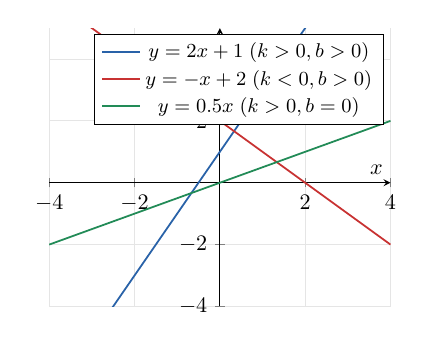
\begin{tikzpicture}[scale=0.8]
\begin{axis}[
  axis lines=middle,
  xlabel=$x$, ylabel=$y$,
  xmin=-4, xmax=4, ymin=-4, ymax=5,
  width=7cm, height=6cm,
  grid=both,
  grid style={gray!20},
  legend style={at={(0.98,0.98)}, anchor=north east, font=\small}
]
\addplot[mainblue, thick, domain=-4:4, samples=2] {2*x+1};
\addlegendentry{$y=2x+1\;(k>0,b>0)$}
\addplot[warnred, thick, domain=-4:4, samples=2] {-x+2};
\addlegendentry{$y=-x+2\;(k<0,b>0)$}
\addplot[tipgreen, thick, domain=-4:4, samples=2] {0.5*x};
\addlegendentry{$y=0.5x\;(k>0,b=0)$}
\end{axis}
\end{tikzpicture}
\end{center}

% -------------------- 1.5 反比例函数 --------------------
\subsection*{1.5\quad 反比例函数 $y = \dfrac{k}{x}$ 回顾}

\begin{knowledgebox}[反比例函数的图象与性质]
反比例函数 $y = \dfrac{k}{x}$（$k \neq 0$）的图象是\textbf{双曲线}。
\begin{itemize}[leftmargin=2em]
  \item $k > 0$：图象在第一、三象限，在每个象限内 $y$ 随 $x$ 增大而\textbf{减小}；
  \item $k < 0$：图象在第二、四象限，在每个象限内 $y$ 随 $x$ 增大而\textbf{增大}。
\end{itemize}
\textbf{注意}：$x \neq 0$（$y$ 轴是渐近线），图象无限接近坐标轴但不与坐标轴相交。
\end{knowledgebox}

\begin{center}
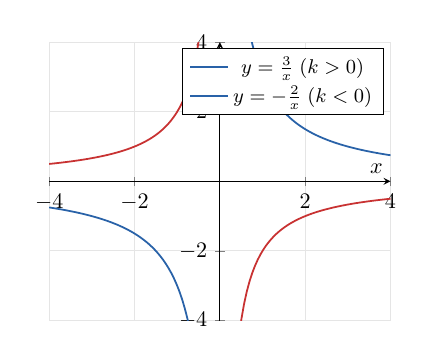
\begin{tikzpicture}[scale=0.8]
\begin{axis}[
  axis lines=middle,
  xlabel=$x$, ylabel=$y$,
  xmin=-4, xmax=4, ymin=-4, ymax=4,
  width=7cm, height=6cm,
  grid=both,
  grid style={gray!20},
  legend style={at={(0.98,0.98)}, anchor=north east, font=\small}
]
\addplot[mainblue, thick, domain=0.25:4, samples=60] {3/x};
\addplot[mainblue, thick, domain=-4:-0.25, samples=60] {3/x};
\addlegendentry{$y=\frac{3}{x}\;(k>0)$}
\addplot[warnred, thick, domain=0.25:4, samples=60] {-2/x};
\addplot[warnred, thick, domain=-4:-0.25, samples=60] {-2/x};
\addlegendentry{$y=-\frac{2}{x}\;(k<0)$}
\end{axis}
\end{tikzpicture}
\end{center}

% -------------------- 1.6 二次函数图象回顾 --------------------
\subsection*{1.6\quad 二次函数图象回顾}

\begin{knowledgebox}[二次函数 $y = ax^2 + bx + c$]
二次函数的图象是\textbf{抛物线}。
\begin{itemize}[leftmargin=2em]
  \item $a > 0$：开口\textbf{向上}，有最低点（最小值）；
  \item $a < 0$：开口\textbf{向下}，有最高点（最大值）；
  \item $|a|$ 越大，抛物线开口越\textbf{窄}。
\end{itemize}

\textbf{顶点坐标}：
\[
  \text{顶点} = \left(-\frac{b}{2a},\;\frac{4ac - b^2}{4a}\right)
\]

\textbf{对称轴}：$x = -\dfrac{b}{2a}$。
\end{knowledgebox}

\begin{center}
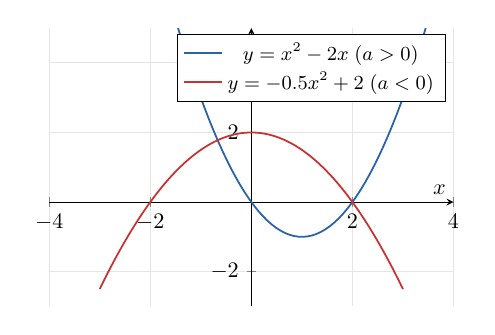
\begin{tikzpicture}[scale=0.8]
\begin{axis}[
  axis lines=middle,
  xlabel=$x$, ylabel=$y$,
  xmin=-4, xmax=4, ymin=-3, ymax=5,
  width=8cm, height=6cm,
  grid=both,
  grid style={gray!20},
  legend style={at={(0.98,0.98)}, anchor=north east, font=\small}
]
\addplot[mainblue, thick, domain=-3.5:3.5, samples=80] {x^2-2*x};
\addlegendentry{$y=x^2-2x\;(a>0)$}
\addplot[warnred, thick, domain=-3:3, samples=80] {-0.5*x^2+2};
\addlegendentry{$y=-0.5x^2+2\;(a<0)$}
\end{axis}
\end{tikzpicture}
\end{center}

% -------------------- 1.7 函数的单调性 --------------------
\subsection*{1.7\quad 函数的单调性（预习高中）}

\begin{knowledgebox}[单调性——描述 $y$ 随 $x$ 变化的趋势]
\textbf{增函数}：在某个范围内，$x$ 增大时 $y$ 也随之增大（图象从左到右\textbf{上升}）。\\
\textbf{减函数}：在某个范围内，$x$ 增大时 $y$ 反而减小（图象从左到右\textbf{下降}）。

用更严格的语言表述（高中定义）：
\begin{itemize}[leftmargin=2em]
  \item 设 $x_1 < x_2$，若 $f(x_1) < f(x_2)$，则 $f(x)$ 在该区间上是\textbf{增函数}；
  \item 设 $x_1 < x_2$，若 $f(x_1) > f(x_2)$，则 $f(x)$ 在该区间上是\textbf{减函数}。
\end{itemize}

\textbf{判断方法（图象法）}：从左往右看图象，上升即增，下降即减。
\end{knowledgebox}

\begin{tipbox}[常见函数的单调性]
\begin{itemize}[leftmargin=2em]
  \item $y = 2x + 1$：在 $(-\infty, +\infty)$ 上单调递增；
  \item $y = -x + 3$：在 $(-\infty, +\infty)$ 上单调递减；
  \item $y = x^2$：在 $(-\infty, 0)$ 上单调递减，在 $(0, +\infty)$ 上单调递增；
  \item $y = \dfrac{1}{x}$：在 $(-\infty, 0)$ 和 $(0, +\infty)$ 上分别单调递减（注意：不能说在整个定义域上递减）。
\end{itemize}
\end{tipbox}

% -------------------- 1.8 函数的奇偶性 --------------------
\subsection*{1.8\quad 函数的奇偶性预习（简单介绍）}

\begin{knowledgebox}[奇函数与偶函数]
设函数 $f(x)$ 的定义域关于原点对称，即 $x$ 和 $-x$ 都在定义域内。

\textbf{偶函数}：若 $f(-x) = f(x)$，则 $f(x)$ 是偶函数。\\
图象特征：关于\textbf{$y$ 轴}对称。\\
例如：$y = x^2$，$y = |x|$。

\textbf{奇函数}：若 $f(-x) = -f(x)$，则 $f(x)$ 是奇函数。\\
图象特征：关于\textbf{原点}对称。\\
例如：$y = x$，$y = x^3$，$y = \dfrac{1}{x}$。
\end{knowledgebox}

\begin{center}
\begin{tikzpicture}[scale=0.75]
\begin{axis}[
  axis lines=middle,
  xlabel=$x$, ylabel=$y$,
  xmin=-3.5, xmax=3.5, ymin=-1, ymax=5,
  width=7cm, height=5.5cm,
  grid=both,
  grid style={gray!20},
  title={\textbf{偶函数 $y=x^2$（关于 $y$ 轴对称）}},
  title style={font=\small}
]
\addplot[mainblue, thick, domain=-3:3, samples=60] {x^2};
\draw[dashed, tipgreen] (axis cs:0,0) -- (axis cs:0,5);
\end{axis}
\end{tikzpicture}
\hspace{1cm}
\begin{tikzpicture}[scale=0.75]
\begin{axis}[
  axis lines=middle,
  xlabel=$x$, ylabel=$y$,
  xmin=-3.5, xmax=3.5, ymin=-3.5, ymax=3.5,
  width=7cm, height=5.5cm,
  grid=both,
  grid style={gray!20},
  title={\textbf{奇函数 $y=x^3$（关于原点对称）}},
  title style={font=\small}
]
\addplot[mainblue, thick, domain=-1.5:1.5, samples=60] {x^3};
\draw[dashed, tipgreen] (axis cs:0,-3.5) -- (axis cs:0,3.5);
\end{axis}
\end{tikzpicture}
\end{center}

% ===========================================================
%   第二部分：例题精讲
% ===========================================================
\section*{\textcolor{examorange}{二、例题精讲}}

% ---- 例题1 ----
\begin{examplebox}[【例题1】坐标系基础——求点的坐标与象限]
已知点 $A(3,-2)$，$B(-1,4)$，$C(0,-5)$，$D(-3,0)$。
\begin{enumerate}[label=(\arabic*)]
  \item 指出各点分别在哪个象限或坐标轴上；
  \item 求点 $A$ 关于 $x$ 轴、$y$ 轴、原点的对称点坐标。
\end{enumerate}
\end{examplebox}

\textbf{解}：
\begin{enumerate}[label=(\arabic*)]
  \item $A(3,-2)$：$x>0,\,y<0$，在\textbf{第四象限}；\\
        $B(-1,4)$：$x<0,\,y>0$，在\textbf{第二象限}；\\
        $C(0,-5)$：$x=0$，在\textbf{$y$ 轴上}；\\
        $D(-3,0)$：$y=0$，在\textbf{$x$ 轴上}。
  \item $A(3,-2)$：
        \begin{itemize}
          \item 关于 $x$ 轴对称：$(3,\,2)$；
          \item 关于 $y$ 轴对称：$(-3,\,-2)$；
          \item 关于原点对称：$(-3,\,2)$。
        \end{itemize}
\end{enumerate}

% ---- 例题2 ----
\begin{examplebox}[【例题2】函数概念辨析]
下列各关系中，$y$ 是否是 $x$ 的函数？说明理由。
\begin{enumerate}[label=(\arabic*)]
  \item $y = 3x - 1$
  \item $y^2 = x \quad (x \geqslant 0)$
  \item $|y| = x$
  \item 如图，用图象表示 $y$ 与 $x$ 的关系（一条竖直线与 $y$ 轴平行）
\end{enumerate}
\end{examplebox}

\textbf{解}：
\begin{enumerate}[label=(\arabic*)]
  \item $y = 3x - 1$：对每一个 $x$，$y$ 有唯一确定的值。\textbf{是函数}。
  \item $y^2 = x$：当 $x=4$ 时，$y=2$ 或 $y=-2$（两个值）。\textbf{不是函数}。
  \item $|y| = x$：当 $x=4$ 时，$y=4$ 或 $y=-4$。\textbf{不是函数}。
  \item 竖直线：一个 $x$ 对应多个 $y$。\textbf{不是函数}。
\end{enumerate}

\begin{tipbox}[判断关键]
一个 $x$ 对应\textbf{唯一}的 $y$ $\Rightarrow$ 是函数。一个 $x$ 对应\textbf{多个} $y$ $\Rightarrow$ 不是函数。但多个 $x$ 对应同一个 $y$，\textbf{可以}是函数。
\end{tipbox}

% ---- 例题3 ----
\begin{examplebox}[【例题3】求函数的定义域]
求下列函数的定义域：
\begin{enumerate}[label=(\arabic*)]
  \item $y = 2x + 3$
  \item $y = \dfrac{1}{x - 2}$
  \item $y = \sqrt{x - 1}$
  \item $y = \dfrac{\sqrt{x+2}}{x}$
\end{enumerate}
\end{examplebox}

\textbf{解}：
\begin{enumerate}[label=(\arabic*)]
  \item $y = 2x + 3$：$x$ 取全体实数。定义域为 $\mathbb{R}$（即 $(-\infty, +\infty)$）。
  \item $y = \dfrac{1}{x-2}$：分母不能为零，$x - 2 \neq 0$，即 $x \neq 2$。\\
        定义域为 $\{x \mid x \neq 2\}$，即 $(-\infty, 2) \cup (2, +\infty)$。
  \item $y = \sqrt{x-1}$：被开方数 $\geqslant 0$，$x - 1 \geqslant 0$，即 $x \geqslant 1$。\\
        定义域为 $[1, +\infty)$。
  \item $y = \dfrac{\sqrt{x+2}}{x}$：同时满足 $x + 2 \geqslant 0$ 且 $x \neq 0$。\\
        即 $x \geqslant -2$ 且 $x \neq 0$。定义域为 $[-2,\,0) \cup (0, +\infty)$。
\end{enumerate}

% ---- 例题4 ----
\begin{examplebox}[【例题4】判断函数图象]
下列各图中，哪个图象能表示 $y$ 是 $x$ 的函数？

\begin{center}
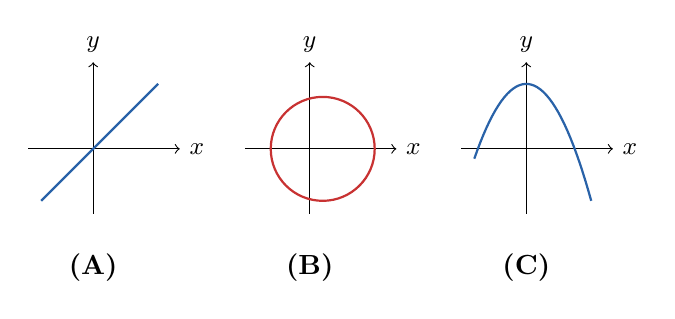
\begin{tikzpicture}[scale=0.55]
% A: 直线（是函数）
\begin{scope}[shift={(0,0)}]
  \draw[->] (-1.5,0) -- (2,0) node[right]{\small$x$};
  \draw[->] (0,-1.5) -- (0,2) node[above]{\small$y$};
  \draw[mainblue, thick] (-1.2,-1.2) -- (1.5,1.5);
  \node[below] at (0,-2.2) {\textbf{(A)}};
\end{scope}
% B: 圆（不是函数）
\begin{scope}[shift={(5,0)}]
  \draw[->] (-1.5,0) -- (2,0) node[right]{\small$x$};
  \draw[->] (0,-1.5) -- (0,2) node[above]{\small$y$};
  \draw[warnred, thick] (0.3,0) circle(1.2);
  \node[below] at (0,-2.2) {\textbf{(B)}};
\end{scope}
% C: 抛物线（是函数）
\begin{scope}[shift={(10,0)}]
  \draw[->] (-1.5,0) -- (2,0) node[right]{\small$x$};
  \draw[->] (0,-1.5) -- (0,2) node[above]{\small$y$};
  \draw[mainblue, thick, domain=-1.2:1.5, samples=40] plot (\x, {1.5-1.2*\x*\x});
  \node[below] at (0,-2.2) {\textbf{(C)}};
\end{scope}
\end{tikzpicture}
\end{center}
\end{examplebox}

\textbf{解}：
\textbf{(A)} 是函数（每个 $x$ 对应唯一 $y$）；\\
\textbf{(B)} 不是函数（例如 $x=0.3$ 时对应两个 $y$ 值）；\\
\textbf{(C)} 是函数（每个 $x$ 对应唯一 $y$）。

\begin{tipbox}[竖直线检验法]
在图象上任意画一条与 $y$ 轴平行的直线，若该直线与图象至多有\textbf{一个}交点，则该图象表示函数（这叫"竖直线检验法"）。
\end{tipbox}

% ---- 例题5 ----
\begin{examplebox}[【例题5】从图象读信息]
小明骑自行车从家出发去图书馆，下图表示他离家的距离 $s$（千米）与时间 $t$（分钟）的关系。
\begin{center}
\begin{tikzpicture}[scale=0.7]
\begin{axis}[
  axis lines=left,
  xlabel={\small 时间 $t$（分钟）},
  ylabel={\small 距离 $s$（千米）},
  xmin=0, xmax=50, ymin=0, ymax=3.5,
  width=10cm, height=5cm,
  grid=both,
  grid style={gray!20},
  xtick={0,10,20,30,40,50},
  ytick={0,1,2,3},
]
\addplot[mainblue, very thick] coordinates {
  (0,0) (10,2) (20,2) (30,2) (40,3.2) (50,3.2)
};
\node[above, font=\small] at (axis cs:5,1){\textcircled{1}};
\node[above, font=\small] at (axis cs:25,2.15){\textcircled{2}};
\node[above, font=\small] at (axis cs:35,2.5){\textcircled{3}};
\node[above, font=\small] at (axis cs:45,3.35){\textcircled{4}};
\end{axis}
\end{tikzpicture}
\end{center}
根据图象回答：
\begin{enumerate}[label=(\arabic*)]
  \item 图书馆离家多远？
  \item 小明在途中停留了多长时间？
  \item 哪段路程行驶速度最快？
\end{enumerate}
\end{examplebox}

\textbf{解}：
\begin{enumerate}[label=(\arabic*)]
  \item 图象最终稳定在 $s=3.2$ 千米，图书馆离家 \textbf{3.2 千米}。
  \item 第 10 分钟到第 30 分钟，$s$ 没有变化（图象水平），停留了 $30-10=20$ \textbf{分钟}。
  \item 比较各段斜率（即速度）：
        \begin{itemize}
          \item 段 $\textcircled{1}$（$0\sim10$ 分钟）：$v=\dfrac{2}{10}=0.2$ 千米/分钟；
          \item 段 $\textcircled{3}$（$30\sim40$ 分钟）：$v=\dfrac{3.2-2}{10}=0.12$ 千米/分钟。
        \end{itemize}
        段 $\textcircled{1}$ 的速度最快，为 \textbf{0.2 千米/分钟}。
\end{enumerate}

% ---- 例题6 ----
\begin{examplebox}[【例题6】一次函数综合]
已知一次函数 $y = kx + b$ 的图象经过点 $A(1, 3)$ 和 $B(-1, -1)$。
\begin{enumerate}[label=(\arabic*)]
  \item 求 $k$ 和 $b$ 的值；
  \item 求该函数图象与 $x$ 轴、$y$ 轴的交点坐标；
  \item 判断该函数的单调性。
\end{enumerate}
\end{examplebox}

\textbf{解}：
\begin{enumerate}[label=(\arabic*)]
  \item 将 $A(1,3)$ 和 $B(-1,-1)$ 代入 $y = kx + b$：
        \[
          \begin{cases} k \cdot 1 + b = 3 \\ k \cdot (-1) + b = -1 \end{cases}
          \quad\Rightarrow\quad
          \begin{cases} k + b = 3 \\ -k + b = -1 \end{cases}
        \]
        两式相加：$2b = 2$，$b = 1$；代入得 $k = 2$。
        所以 $y = 2x + 1$。
  \item 与 $y$ 轴交点：令 $x=0$，$y=1$，交点为 $(0,\,1)$。\\
        与 $x$ 轴交点：令 $y=0$，$2x+1=0$，$x=-\dfrac{1}{2}$，交点为 $\left(-\dfrac{1}{2},\,0\right)$。
  \item $k = 2 > 0$，该函数在 $(-\infty, +\infty)$ 上\textbf{单调递增}。
\end{enumerate}

% ---- 例题7 ----
\begin{examplebox}[【例题7】函数与方程、不等式的关系]
已知一次函数 $y = 2x - 4$ 的图象如下：
\begin{center}
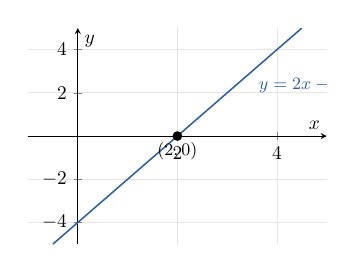
\begin{tikzpicture}[scale=0.7]
\begin{axis}[
  axis lines=middle,
  xlabel=$x$, ylabel=$y$,
  xmin=-1, xmax=5, ymin=-5, ymax=5,
  width=7cm, height=5.5cm,
  grid=both,
  grid style={gray!20},
]
\addplot[mainblue, thick, domain=-0.5:4.5, samples=2] {2*x-4};
\node[below right, font=\small, mainblue] at (axis cs:3.5,3){$y=2x-4$};
\fill (axis cs:2,0) circle(2.5pt) node[below]{\small$(2,0)$};
\end{axis}
\end{tikzpicture}
\end{center}
\begin{enumerate}[label=(\arabic*)]
  \item 求方程 $2x - 4 = 0$ 的解（从图象上看）；
  \item 求不等式 $2x - 4 > 0$ 的解集（从图象上看）；
  \item 当 $x$ 取何值时，$y < 0$？
\end{enumerate}
\end{examplebox}

\textbf{解}：
\begin{enumerate}[label=(\arabic*)]
  \item $2x - 4 = 0$，即 $y = 0$，图象与 $x$ 轴交于 $x=2$。\\
        方程的解为 $x = 2$。
  \item $2x - 4 > 0$，即 $y > 0$，图象在 $x$ 轴上方时 $x > 2$。\\
        解集为 $x > 2$。
  \item $y < 0$，即图象在 $x$ 轴下方，此时 $x < 2$。
\end{enumerate}

\begin{tipbox}[函数与方程、不等式]
\begin{itemize}[leftmargin=2em]
  \item $f(x) = 0$ 的解 $\Leftrightarrow$ 图象与 $x$ 轴交点的横坐标；
  \item $f(x) > 0$ 的解集 $\Leftrightarrow$ 图象在 $x$ 轴\textbf{上方}的部分对应的 $x$ 范围；
  \item $f(x) < 0$ 的解集 $\Leftrightarrow$ 图象在 $x$ 轴\textbf{下方}的部分对应的 $x$ 范围。
\end{itemize}
这是高中"数形结合"思想的重要基础！
\end{tipbox}

% ---- 例题8 ----
\begin{examplebox}[【例题8】函数单调性判断（图象法）]
观察下列函数图象，指出各函数在哪些区间上单调递增、哪些区间上单调递减。

\begin{center}
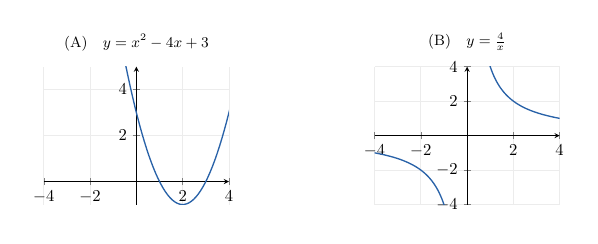
\begin{tikzpicture}[scale=0.6]
% 图1: 二次函数
\begin{scope}[shift={(0,0)}]
  \begin{axis}[
    axis lines=middle,
    xmin=-4, xmax=4, ymin=-1, ymax=5,
    width=5.5cm, height=4.5cm,
    grid=both, grid style={gray!15},
    title={(A)\quad $y=x^2-4x+3$}, title style={font=\small},
    xtick={-4,-2,...,4}, ytick={0,2,4},
  ]
  \addplot[mainblue, thick, domain=-3:5, samples=80] {x^2-4*x+3};
  \end{axis}
\end{scope}
% 图2: 反比例
\begin{scope}[shift={(7,0)}]
  \begin{axis}[
    axis lines=middle,
    xmin=-4, xmax=4, ymin=-4, ymax=4,
    width=5.5cm, height=4.5cm,
    grid=both, grid style={gray!15},
    title={(B)\quad $y=\frac{4}{x}$}, title style={font=\small},
    xtick={-4,-2,...,4}, ytick={-4,-2,...,4},
  ]
  \addplot[mainblue, thick, domain=0.5:4, samples=60] {4/x};
  \addplot[mainblue, thick, domain=-4:-0.5, samples=60] {4/x};
  \end{axis}
\end{scope}
\end{tikzpicture}
\end{center}
\end{examplebox}

\textbf{解}：

\textbf{(A)} $y = x^2 - 4x + 3$，顶点在 $x = 2$ 处。
\begin{itemize}
  \item 在 $(-\infty,\,2)$ 上单调递减（图象从左到右下降）；
  \item 在 $(2,\,+\infty)$ 上单调递增（图象从左到右上升）。
\end{itemize}

\textbf{(B)} $y = \dfrac{4}{x}$，$k = 4 > 0$。
\begin{itemize}
  \item 在 $(-\infty,\,0)$ 上单调递减；
  \item 在 $(0,\,+\infty)$ 上单调递减。
\end{itemize}
注意：不能说"在 $(-\infty, 0) \cup (0, +\infty)$ 上单调递减"，因为取 $x_1=-1,\,x_2=1$ 时 $x_1 < x_2$ 但 $f(x_1)=-4 < 4=f(x_2)$，并不递减。必须分开说每个区间。

% ===========================================================
%   第三部分：应用题
% ===========================================================
\section*{\textcolor{apppurple}{三、应用题}}

% ---- 应用1 ----
\begin{appbox}[【应用1】出租车计费问题]
某市出租车的收费标准为：起步价 8 元（含 3 千米），超过 3 千米后每千米加收 2 元（不足 1 千米按 1 千米计算）。
\begin{enumerate}[label=(\arabic*)]
  \item 写出行驶 $x$ 千米（$x > 3$）时车费 $y$（元）与 $x$ 的函数关系式；
  \item 小明乘坐出租车行驶了 10 千米，应付多少元？
\end{enumerate}
\end{appbox}

\textbf{解}：
\begin{enumerate}[label=(\arabic*)]
  \item 超过 3 千米的部分为 $(x - 3)$ 千米，每千米 2 元。
        \[
          y = 8 + 2(x - 3) = 2x + 2 \quad (x > 3)
        \]
  \item $x = 10$ 时，$y = 2 \times 10 + 2 = 22$ 元。
\end{enumerate}

% ---- 应用2 ----
\begin{appbox}[【应用2】手机话费方案选择]
某通信公司提供两种手机话费套餐：\\
套餐 A：月租 28 元，通话每分钟 0.15 元；\\
套餐 B：月租 58 元，通话每分钟 0.08 元。
\begin{enumerate}[label=(\arabic*)]
  \item 分别写出两种套餐月话费 $y$（元）与通话时间 $x$（分钟）的函数关系式；
  \item 每月通话多少分钟时，两种套餐费用相同？
  \item 若每月通话 600 分钟，应选哪种套餐更划算？
\end{enumerate}
\end{appbox}

\textbf{解}：
\begin{enumerate}[label=(\arabic*)]
  \item 套餐 A：$y_A = 28 + 0.15x$；\\
        套餐 B：$y_B = 58 + 0.08x$。
  \item 令 $y_A = y_B$：
        \[
          28 + 0.15x = 58 + 0.08x \quad\Rightarrow\quad 0.07x = 30 \quad\Rightarrow\quad x \approx 429 \text{（分钟）}
        \]
        每月通话约 429 分钟时费用相同。
  \item $x = 600$ 时，$y_A = 28 + 0.15 \times 600 = 118$ 元；\\
        $y_B = 58 + 0.08 \times 600 = 106$ 元。\\
        $106 < 118$，选\textbf{套餐 B} 更划算。
\end{enumerate}

% ---- 应用3 ----
\begin{appbox}[【应用3】抛物线型拱桥]
一座抛物线型拱桥的桥拱跨度为 20 米，拱高为 4 米。以桥面（水平方向）为 $x$ 轴，以拱顶为原点建立坐标系（$x$ 轴水平，$y$ 轴竖直向下为正）。
\begin{enumerate}[label=(\arabic*)]
  \item 求拱桥所在抛物线的解析式；
  \item 在距离拱顶水平距离为 6 米处，拱的高度是多少米？
\end{enumerate}
\end{appbox}

\textbf{解}：
\begin{enumerate}[label=(\arabic*)]
  \item 桥拱跨度 20 米，拱高 4 米。以拱顶为原点，$y$ 轴向下为正。\\
        拱桥两端点坐标为 $(-10,\,4)$ 和 $(10,\,4)$，拱顶为 $(0,\,0)$。\\
        设抛物线为 $y = ax^2$（过原点，对称于 $y$ 轴）。\\
        代入 $(10,\,4)$：$4 = a \times 100$，$a = \dfrac{1}{25}$。\\
        所以 $y = \dfrac{1}{25}x^2$（其中 $-10 \leqslant x \leqslant 10$）。
  \item $x = 6$ 时，$y = \dfrac{1}{25} \times 36 = 1.44$ 米。\\
        即距离拱顶水平距离 6 米处，拱高为 \textbf{1.44 米}。
\end{enumerate}

% ===========================================================
%   第四部分：课堂练习
% ===========================================================
\section*{\textcolor{tipgreen}{四、课堂练习}}

\begin{enumerate}[label=\textbf{\arabic*.}, leftmargin=2.5em]
  \item 点 $P(-3,\,2)$ 在第几象限？它关于 $x$ 轴、$y$ 轴的对称点分别在第几象限？

  \item 判断下列关系中，$y$ 是否是 $x$ 的函数：
        \begin{enumerate}[label=(\alph*)]
          \item $y = |x| + 1$
          \item $x^2 + y^2 = 1$
          \item $y = \sqrt{2x + 1}$
        \end{enumerate}

  \item 求函数 $y = \dfrac{3}{x + 1}$ 的定义域。

  \item 一次函数 $y = -3x + 6$ 与 $x$ 轴的交点坐标是什么？与 $y$ 轴的交点坐标是什么？

  \item 已知函数 $y = kx$ 的图象经过点 $(2,\,-6)$，求 $k$ 的值，并判断该函数的单调性。

  \item 反比例函数 $y = \dfrac{6}{x}$ 在第一象限内，当 $x$ 增大时 $y$ 如何变化？

  \item 二次函数 $y = -x^2 + 4x - 3$ 的开口方向是什么？顶点坐标是什么？

  \item 根据下图回答：函数 $f(x)$ 在哪个区间上是增函数？在哪个区间上是减函数？

\begin{center}
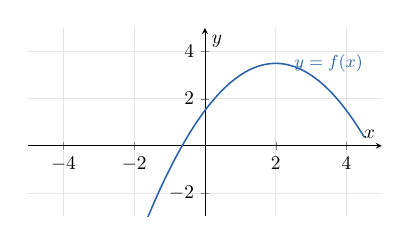
\begin{tikzpicture}[scale=0.7]
\begin{axis}[
  axis lines=middle,
  xlabel=$x$, ylabel=$y$,
  xmin=-5, xmax=5, ymin=-3, ymax=5,
  width=8cm, height=5cm,
  grid=both, grid style={gray!20},
  xtick={-4,-2,0,2,4}, ytick={-2,0,2,4},
]
\addplot[mainblue, thick, domain=-4.5:4.5, samples=100] {-0.5*x^2+2*x+1.5};
\node[mainblue, font=\small] at (axis cs:3.5, 3.5){$y=f(x)$};
\end{axis}
\end{tikzpicture}
\end{center}
\end{enumerate}

% ---- 参考答案 ----
\begin{knowledgebox}[参考答案]
\textbf{1.} $P(-3,2)$ 在第二象限；关于 $x$ 轴对称点 $(-3,-2)$ 在第三象限；关于 $y$ 轴对称点 $(3,2)$ 在第一象限。

\textbf{2.}
\begin{enumerate}[label=(\alph*)]
  \item $y=|x|+1$：是函数（每个 $x$ 对应唯一 $y$）。
  \item $x^2+y^2=1$：不是函数（如 $x=0$ 时 $y=\pm1$，不唯一）。
  \item $y=\sqrt{2x+1}$：是函数（每个 $x$ 对应唯一 $y$）。
\end{enumerate}

\textbf{3.} 分母 $x+1 \neq 0$，即 $x \neq -1$。定义域为 $\{x \mid x \neq -1\}$，即 $(-\infty,-1)\cup(-1,+\infty)$。

\textbf{4.} 与 $x$ 轴交点：令 $y=0$，$-3x+6=0$，$x=2$，交点为 $(2,\,0)$。\\
与 $y$ 轴交点：令 $x=0$，$y=6$，交点为 $(0,\,6)$。

\textbf{5.} $k \cdot 2 = -6$，$k = -3$。函数为 $y = -3x$，$k<0$，在 $(-\infty,+\infty)$ 上单调递减。

\textbf{6.} $k=6>0$，在第一象限（$x>0$）内，$y$ 随 $x$ 增大而减小。

\textbf{7.} $a = -1 < 0$，开口向下。\\
顶点横坐标 $x = -\dfrac{4}{2 \times (-1)} = 2$，纵坐标 $y = -4 + 8 - 3 = 1$。\\
顶点坐标为 $(2,\,1)$。

\textbf{8.} 对称轴 $x = -\dfrac{2}{2\times(-0.5)} = 2$。\\
在 $(-\infty,\,2)$ 上单调递增（图象上升）；\\
在 $(2,\,+\infty)$ 上单调递减（图象下降）。
\end{knowledgebox}

\vfill
\begin{center}
\small\textcolor{gray}{本讲义仅供教学参考，例题可根据学生水平调整难度。}
\end{center}

\end{document}
